\chapter{Methods}

\section{Sampling Images}

The number of images in the NTCIR-12 Lifelog data set far exceeds the possible number of images that can be annotated manually. The collection is very large, containing around 90,000 images. It is certainly unfeasible to annotate every image four times (for each annotation methodology), so sampling images to reduce the number of images to annotate is necessary. There are two methodologies employed to sample images: The first is based off previous work~\cite{scells2016qut} which identifies a way to cluster lifelog images using image histograms for features and aligning the images temporally to determine cluster segmentation points. After clustering images, a this sampling technique involves selecting one image at random from each cluster. The cosine similarity measure is used to determine if an image should be added to an existing cluster. The threshold of the cosine value between two images is set to 0.86\footnote{This value was empirically found to provide a range of sufficiently different clusters, each containing similar images}. Clusters are then combined based on visual similarity using the aforementioned image histograms and a representative image from each of these clusters is chosen at random. This process results in about 16,000 images chosen for annotation. The second sampling method entails processing the qrels to extract only the relevant images. A maximum of 30 images are selected from each topic which results in just over 1,000 images required for annotation (since some topics have less than 30 relevant images, some even having less than 10).
% Given more time, it would be worthwhile investigating other image similarity measures (such as those used by the LEMoRe team at NTCIR-12~\cite{de40lemore}) to possibly produce a more uniformly distributed sample set.

There is some overlap between the images chosen from the clustering process and the images that are known to be relevant, however it reduces the number of images to annotated from 90,000 down to around 16,000. In reality all of the images which are known to be relevant are annotated and around 1,000 from the clustered set of images are annotated. Annotating both relevant and non-relevant images ensures that retrieval is working correctly; both relevant and non-relevant images should be retrieved but the images annotated with relevant annotations should rank higher.

These sampled images are uploaded into a database to be annotated. Annotations are then collected through specially designed interfaces.
% Both sampling techniques are required 
% For future work, a combination of clustering and matching images to relevant topics might be a better option, as there will most likely be many irrelevant annotations. There may also be no annotations which are relevant to a topic as well, since the sampling is somewhat random. This makes the process less than idea, but will serve as a proof of concept for further research.

\section{Collecting Annotations}

Once the images have been sampled and uploaded into a database, they are ready to be annotated. Four web application interfaces are used for the collection of annotations. Each interface provides a means for an annotator to assign the respective annotation type to an image from a list of unannotated images. The architecture of these interfaces consists of:
\begin{enumerate}
    \item A database to store the annotations and the sampled images. The database also stores information about each user performing the annotations, who annotated which image and how long it takes to do an annotation. This ensures there is a record of who annotated each image, and allows for an analysis to be performed at a later stage.
    \item A web server and that handles the `business logic'. This web server exposes some password protected RESTful services that applications can hook into.
    \item A website which consumes the API provided by the web server and handles `view logic'. This is the layer that annotators will interact with directly. Each interface will be one of these views.
\end{enumerate}

Each interface is designed with great care to ensure the collection of annotations is as painless as possible. It is important that the time between annotating one image and starting to annotate the next is as small as possible. If it takes a minute to annotate one image, it will take an hour to annotate only 60 images.

It is for this reason that an automatic captioning system is used to caption the rest of the images. For each methodology, annotations will be generated using a state-of-the-art machine learning architecture. This ensures every single image is annotated, so an annotation has been collected for each image, for each annotation methodology.

\section{Annotation Methodologies}

Four annotation methodologies are selected for investigation: \textbf{textual}, \textbf{tags}, \textbf{relevance assessment} and \textbf{reverse query}. While the annotation types are wildly different to each other, they are all  collected in a very similar way. An expert annotator is shown a randomly chosen image from the sampled set and is asked to provide an annotation (or in the case of relevance assessment, multiple annotations) for the image. The interfaces used for collecting annotations are pictured and described as follows:

\textbf{Textual}

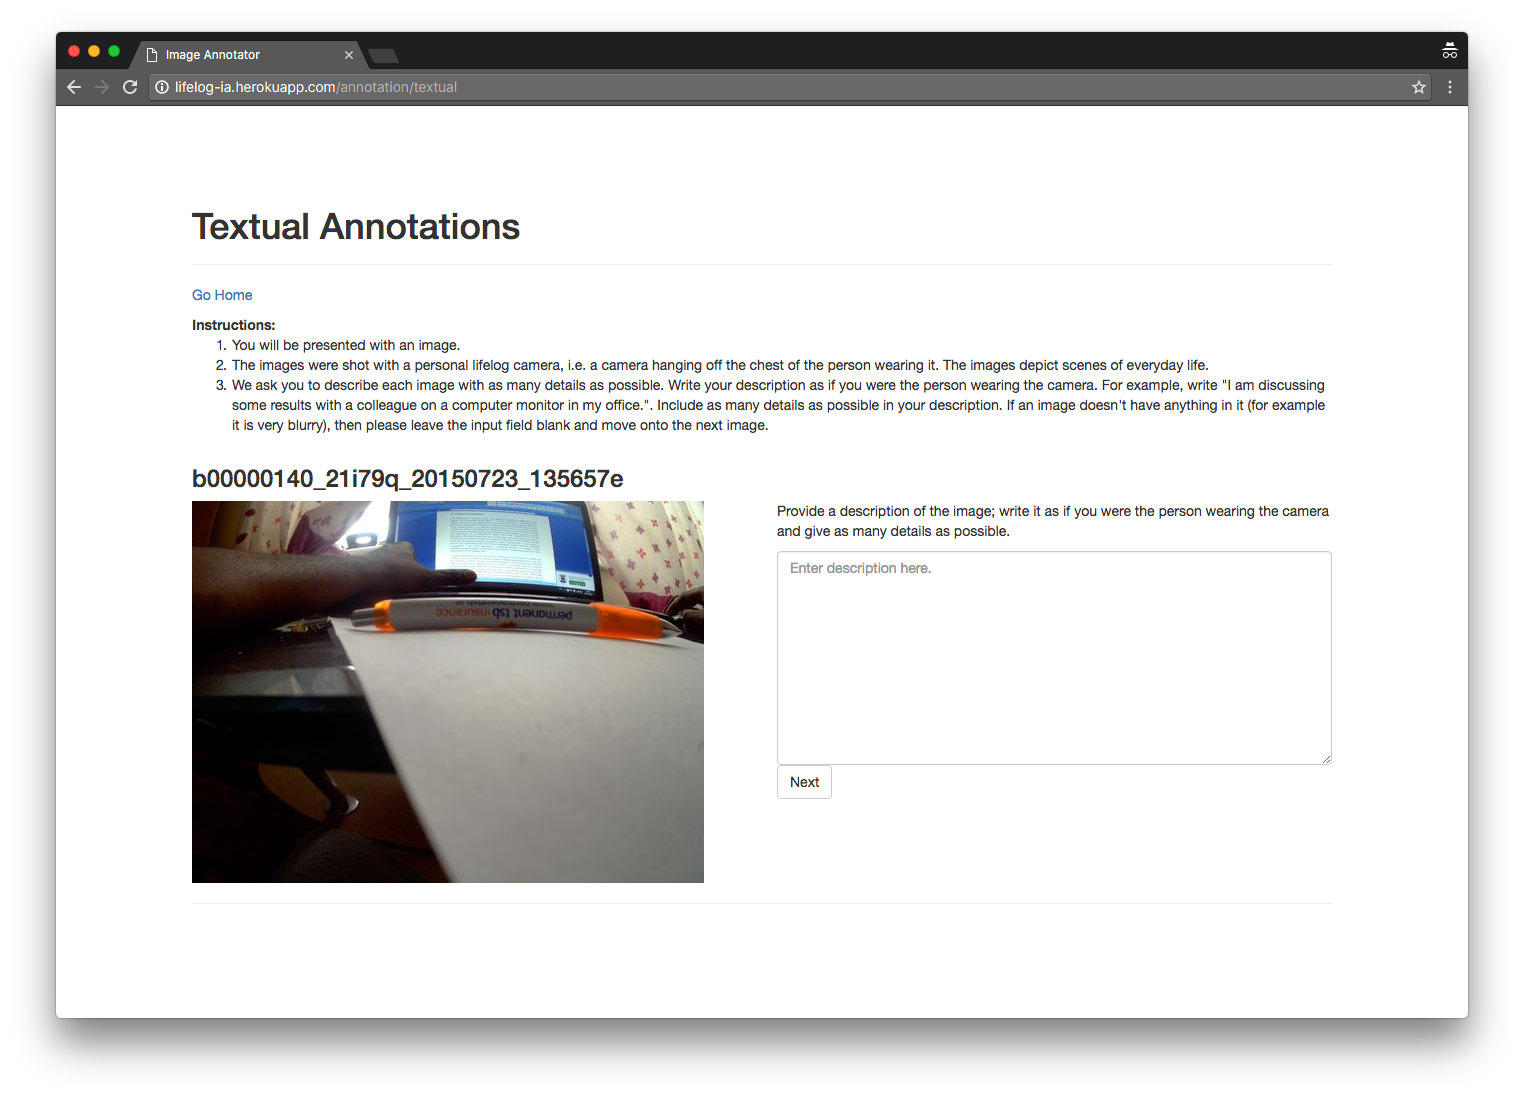
\includegraphics[width=0.95\textwidth]{images/text-interface}

Here, annotations are collected using free form text through a text box on the page. Textual annotations should contain semantic information about an image, and should describe the image with as much detail as possible. These annotations are very similar to a textual document in a typical web search engine, which is why they are selected as one of the methodologies to investigate.

\newpage
\textbf{Tags}

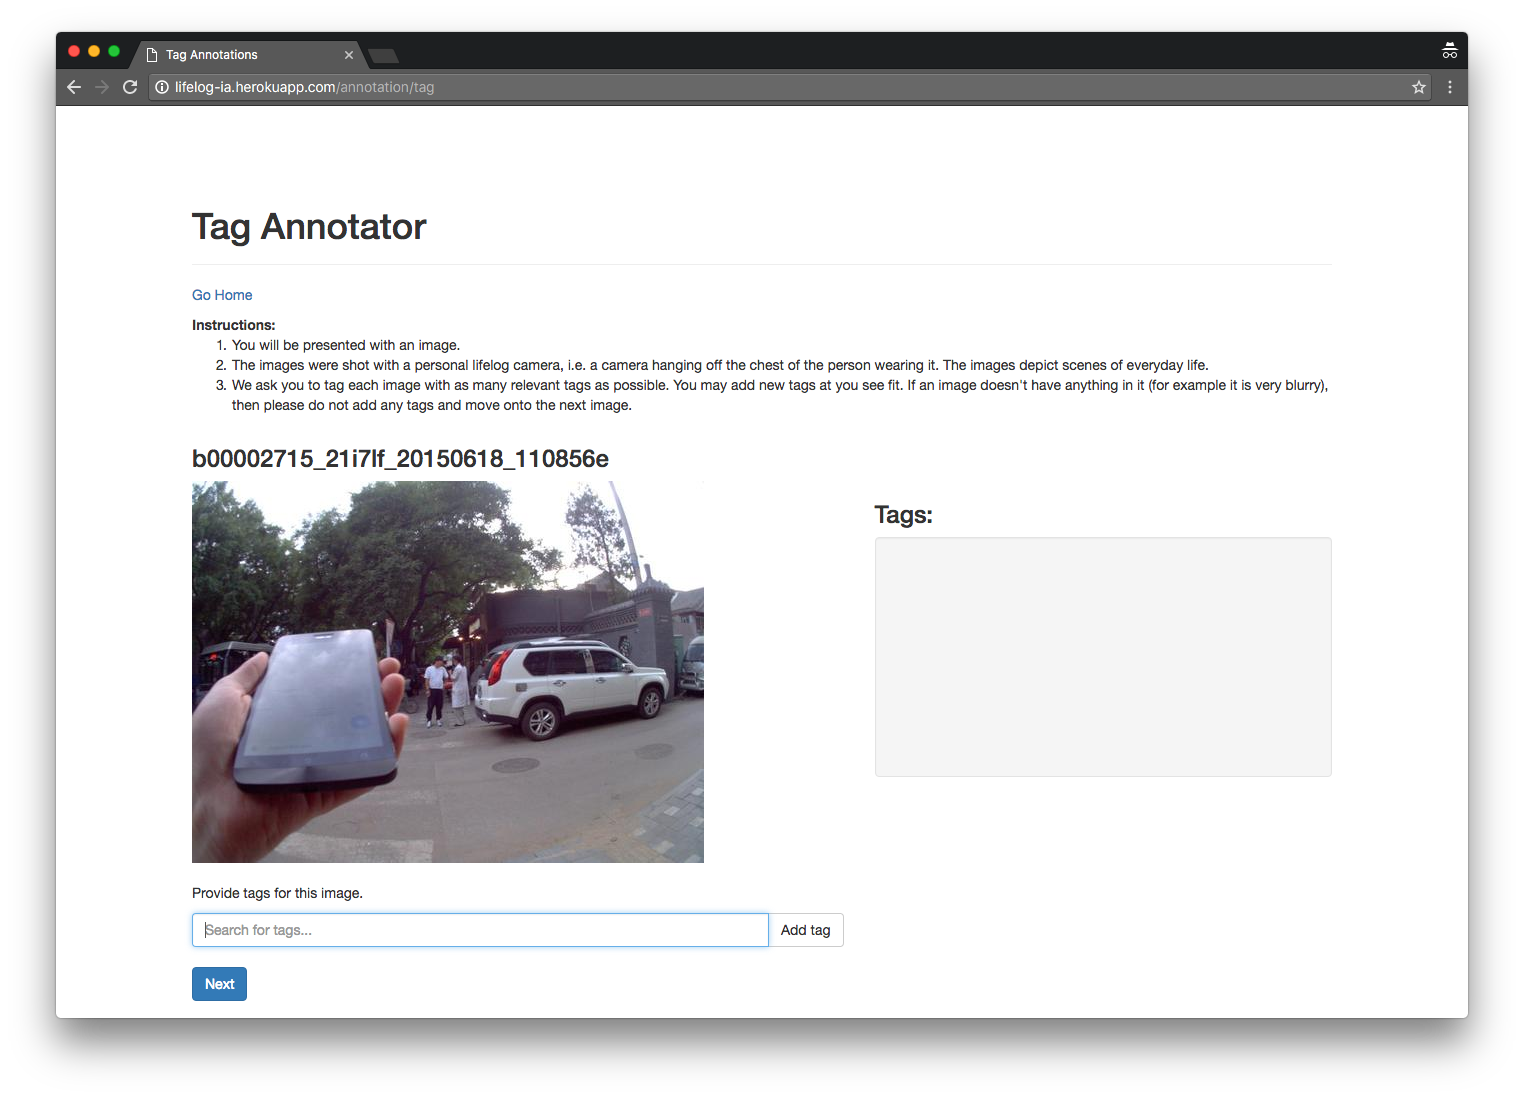
\includegraphics[width=0.95\textwidth]{images/tag-interface}

Tags are collected through a specifically designed interface. These vocabulary of tags is created from previously added tags, meaning the list of tags available is arbitrary and can be expanded. 

\newpage
\textbf{Reverse Query}

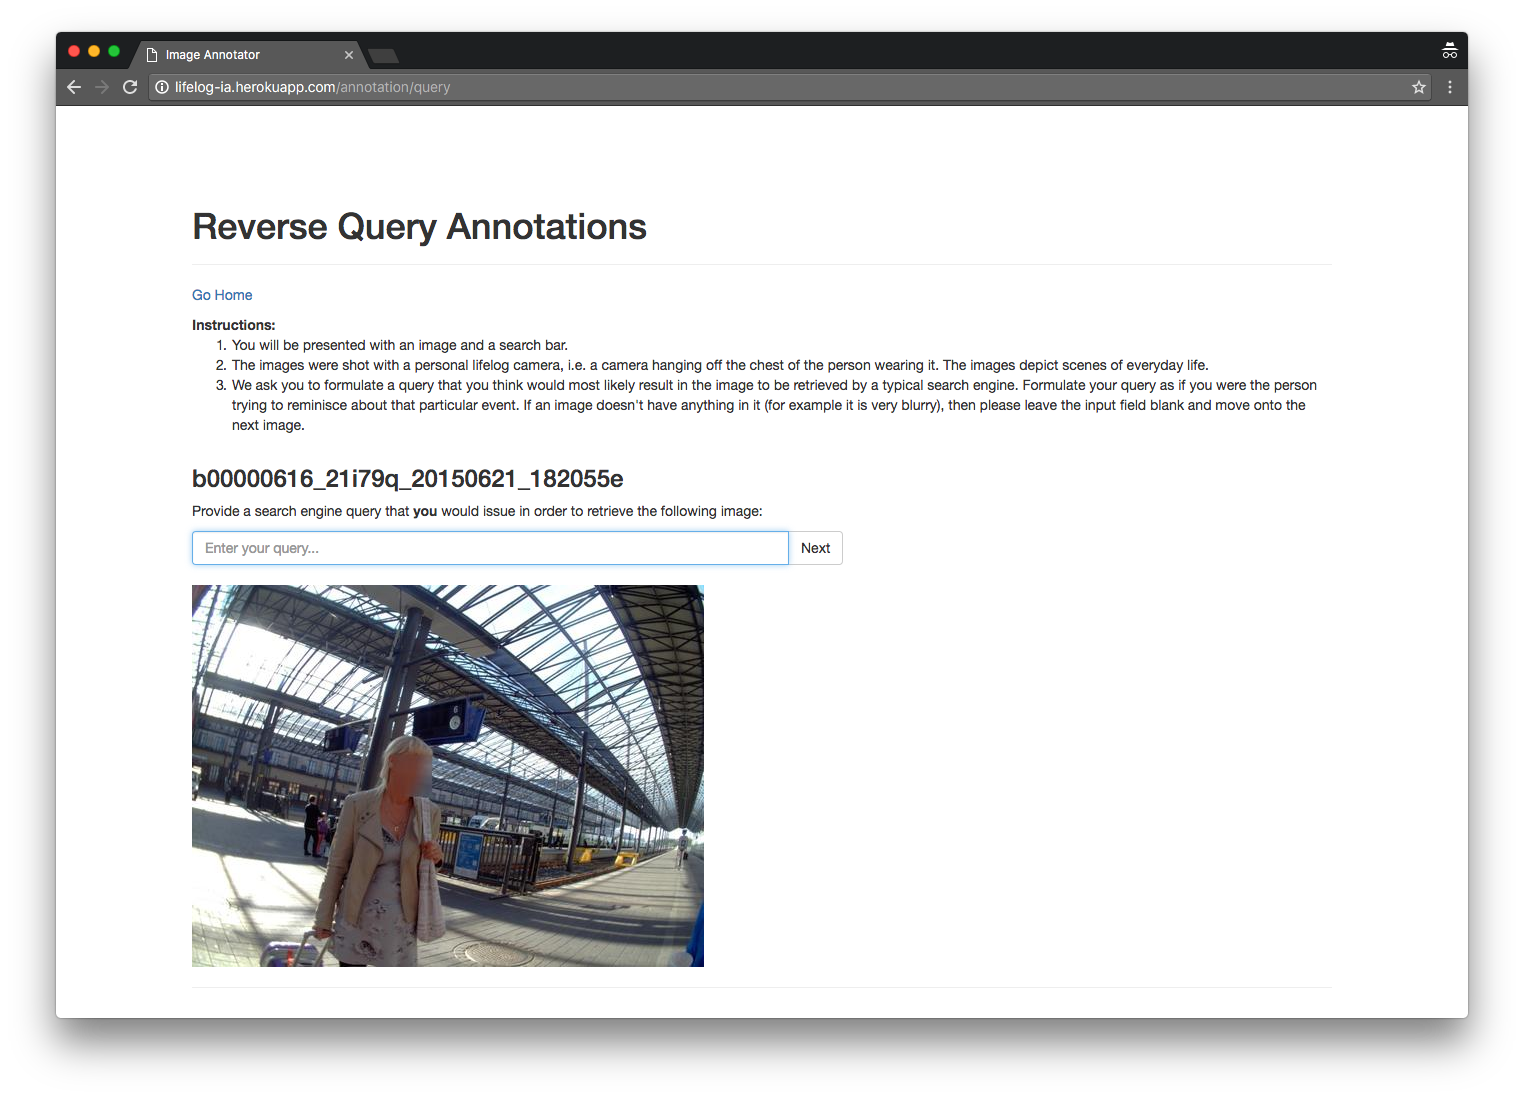
\includegraphics[width=0.95\textwidth]{images/query-interface}

In this interface, user queries are collected by presenting an image taken from the lifelog camera and asking the annotator to provide a query with what they expect to be returned by a typical search engine. This is a relatively new and novel way to annotating \textit{any} type of document or image~\cite{quteprints82599}. 

\newpage
\textbf{Relevance Assessment}

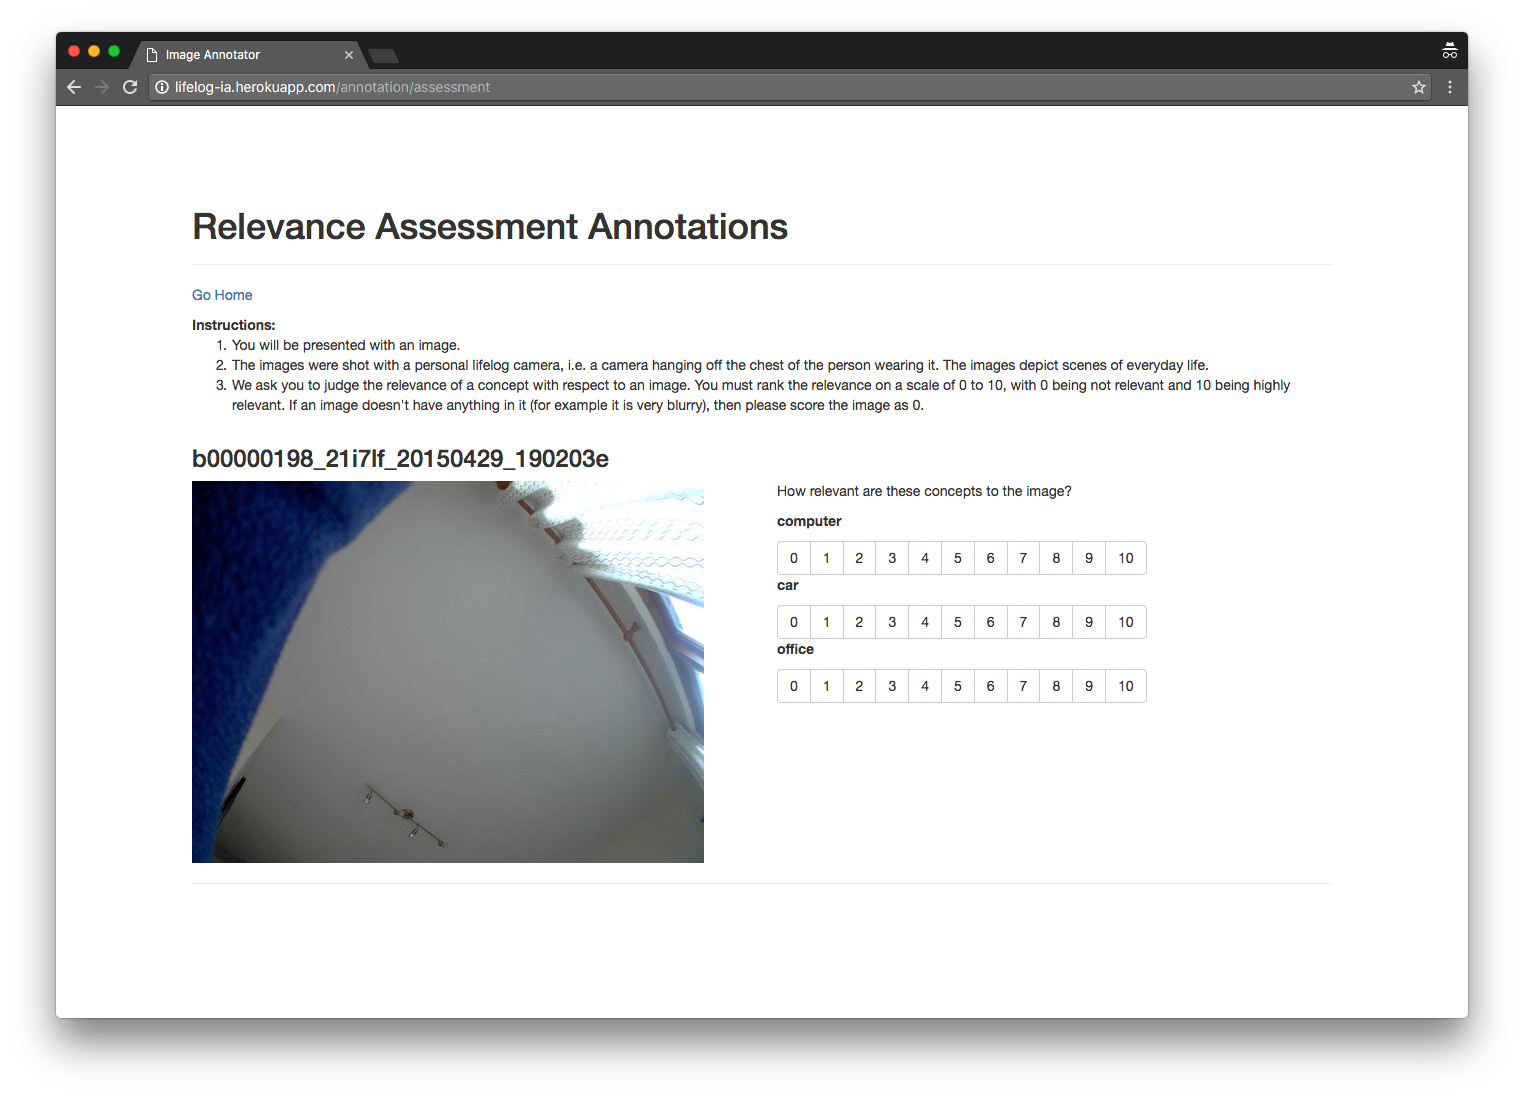
\includegraphics[width=0.95\textwidth]{images/rel-ass-interface}

Relevance assessment involves presenting an annotator with an image, and asking them to judge how relevant a concept is to the image. Assessors are asked to choose concepts from a list to assess, and from those chosen concepts are asked to assess the relevance of that concept to the target image. Concepts are ranked on a scale of zero to ten, where zero is not relevant at all and ten is highly relevant.

These annotations will be collected last, since the list of concepts is formed after analysing the terms. Concepts are chosen by creating a list of terms from the existing textual, tag and query annotations, which are then filtered down to the terms that occur in the NTCIR-12 Lifelog topic titles and descriptions. Each term is then scored using IDF\footnote{Inverse Document Frequency} and then ranked using an algorithm similar to discounted cumulative gain~\cite{jarvelin2002cumulated}; in which higher scoring terms are selected less frequently, and more emphasis is placed on selecting lower scoring terms. 

\newpage
\textbf{Automatic Image Annotation}

Finally, an attempt to automatically caption images for each annotation methodology is done by exploiting a recent state-of-the-art machine learning image captioning approach~\cite{karpathy2015deep} which has been open sourced\footnote{\url{https://github.com/karpathy/neuraltalk2}}. The architecture of the system consists of the final hidden layer of a convolutional neural network (CNN) which learns features of image regions being fed into a recurrent neural network (RNN) that generates textual descriptions.

A model is trained using 70,000 iterations using the $adam$ optimiser with $\alpha$ set to 0.8 and $\beta$ set to 0.999. The learning rate of the language model is set to 0.0004. More iterations are performed afterwards to fine tune the deep learning architecture, but generally insignificant changes if any are seen in the values of the optimisation function.

\section{Evaluating Annotations}

Annotations are evaluated with an ad-hoc, TREC style methodology. The topics and qrels from the NTCIR-12 Lifelog semantic access pilot task are used to perform evaluation. In total eight runs are produced: four consisting of the manually annotated annotations and another four containing the combination of the manually and automatically annotated annotations. This is to find the best annotation methodology - but also to see if automatic annotations can increase the retrieval effectiveness.

Document rankings are generated by submitting queries to ElasticSearch using porter stemmer and a default English stoplist. Queries are formulated by using the title field from the NTCIR-12 Lifelog topics. The stemming and stopping are also applied to the queries. ElasticSearch is also set to only retrieve a maximum of 1,000 images. The runs produced by this system are evaluated using \verb|trec_eval| and the NTCIR-12 Lifelog qrels.

The document rankings and evaluation is performed through a custom-built framework. A Java RESTful application wraps Elasticsearch. This is so a query issued to the Java application can return a properly formatted TREC run, and so many queries can be issued with one request. 
